\chapter{晶体结构\label{ch:1}}

\noindent \textbf{1.\quad} 氯化钠与金刚石型结构是复式格子还是布拉维格子,各自的基元为何?写出这两种结构的原胞与晶胞基矢,设晶格常数为 $a$。

\noindent \textbf{解:}

氯化钠与金刚石型结构都是复式格子。氯化钠的基元为一个 \ce{Na} 用和一个 \ce{Cl} 一组成的正负离子对。金刚石的基元是一个面心立方上的 \ce{C} 原子和一个体对角线上的 \ce{C} 原子组成的 \ce{C} 原子对。

由于 \ce{NaCl} 和金刚石都由面心立方结构套构而成,所以,其\emph{元胞基矢}都为:

\begin{equation*}
    \begin{cases}
        \mathbf{a}_1 = \frac{a}{2} (\mathbf{j} + \mathbf{k}) \\
        \mathbf{a}_2 = \frac{a}{2} (\mathbf{k} + \mathbf{i}) \\
        \mathbf{a}_3 = \frac{a}{2} (\mathbf{i} + \mathbf{j})
    \end{cases}
\end{equation*}

相应的\emph{晶胞基矢}都为:

\begin{equation*}
    \begin{cases}
        \mathbf{a} = a \mathbf{i} \\
        \mathbf{b} = b \mathbf{j} \\
        \mathbf{c} = c \mathbf{k}
    \end{cases}
\end{equation*}

\noindent \textbf{2.\quad} 六角密集结构可取四个原胞基矢 $\mathbf{a}_1, \mathbf{a}_2, \mathbf{a}_3$ 与 $\mathbf{c}$,如图所示。

\begin{figure}[htbp]
    \centering
    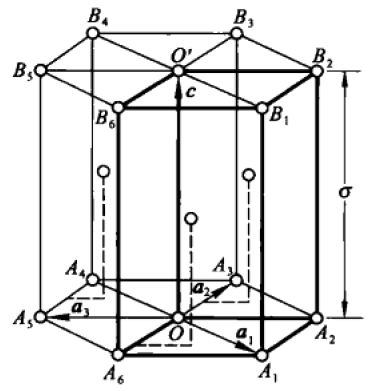
\includegraphics{pic/六方.png}
    \caption{六方}
    \label{fig:1.1}
\end{figure}

\noindent 试写出 $O^\prime A_1 A_3$、$A_1 A_3 B_3 B_1$、$A_2 B_2 B_5 A_5$、$A_1 A_2 A_3 A_4 A_5 A_6$ 这四个面所属晶面族的晶面指数 $(h\ k\ l\ m)$。

\noindent \textbf{解:}

\begin{enumerate}
    \item 对于 $O^\prime A_1 A_3$ 面,其在四个原胞基矢上的截矩分别为:$1, 1, -\frac{1}{2}, 1$。所以,其晶面指数为 $(11\bar{2}1)$。
    \item 对于 $A_1 A_3 B_3 B_1$ 面,其在四个原胞基矢上的截矩分别为:$1, 1, -\frac{1}{2}, \infty$。所以,其晶面指数为 $(11\bar{2}0)$ 。
    \item 对于 $A_2 B_2 B_5 A_5$ 面,其在四个原胞基矢上的截矩分别为:$1, -1, \infty, \infty$。所以,其晶面指数为 $(1\bar{1}00)$。
    \item 对于 $A_1 A_2 A_3 A_4 A_5 A_6$ 面,其在四个原胞基矢上的截矩分别为:$\infty, \infty, \infty, 1$。所以,其晶面指数为 $(0001)$。
\end{enumerate}

\noindent \textbf{3.\quad} 如将等体积的硬球堆成下列结构,求证球体可能占据的最大体积与总体积的比为:简立方:$\frac{\pi}{6}$;体心立方:$\frac{\sqrt{3}\pi}{8}$;面心立方:$\frac{\sqrt{2}\pi}{6}$;六角密集:$\frac{\sqrt{2}\pi}{6}$;金刚石:$\frac{\sqrt{3}\pi}{16}$;

\noindent \textbf{证明:}

由于晶格常数为 $a$, 所以:

构成简立方时,最大球半径为 $R_m=\frac{a}{2}$,每个原胞中占有一个原子,

\begin{align*}
    \therefore V_m &= \frac{4}{3} \pi \left(\frac{a}{2}\right)^3 = \frac{\pi}{6} a^3 \\
    \therefore \frac{V_m}{a^3} &= \frac{\pi}{6}
\end{align*}

构成体心立方时,体对角线等于 $4$ 倍的最大球半径,即:$4 R_m=\sqrt{3} a$,每个晶胞中占有两个原子,

\begin{align*}
    \therefore 2 V_m &= 2 \times \frac{4}{3} \pi \left(\frac{\sqrt{3}}{4} a\right)^3 = \frac{\sqrt{3}\pi}{8} a^3 \\
    \therefore \frac{2 V_m}{a^3} &= \frac{\sqrt{3}\pi}{8}
\end{align*}

构成面心立方时,面对角线等于 $4$ 倍的最大球半径,即:$4 R_m=\sqrt{2}a$ 正每个晶胞占有 $4$ 个原子,

\begin{align*}
    \therefore 4 V_m &= 4 \times \frac{4}{3} \pi \left(\frac{\sqrt{2}}{4} a\right)^3 = \frac{\sqrt{2}\pi}{6} a^3 \\
    \therefore \frac{4 V_m}{a^3} &= \frac{\sqrt{2}\pi}{6}
\end{align*}

构成六角密集结构时,中间层的三个原子与底面中心的那个原子恰构成一个正四面体,其高则正好是其原胞基矢 $c$ 的长度的一半,由几何知识易知 $|c|=-R_m$。原胞底面边长为 $2 R_m$。每个晶胞占有两个原子,

\begin{equation*}
    \therefore 2 V_m = 2 \times \frac{4}{3} \pi R_m^3 = \frac{8}{3} \pi R_m^3
\end{equation*}

原胞的体积为:$V=(2 R_m)^2 \sin \ang{60} \cdot \frac{4\sqrt{6}}{3} R_m = 8\sqrt{2} R_m^3$

\begin{equation*}
    \therefore \frac{2 V_m}{V} = \frac{\pi}{3\sqrt{2}} = \frac{\sqrt{2}\pi}{6}
\end{equation*}

构成金刚石结构时,一的体对角线长度等于两个最大球半径,即:$2 R_m=\frac{\sqrt{3}}{4} a$,每个晶胞包含 $8$ 个原子,

\begin{align*}
    \therefore 8 V_m &= 8 \times \frac{4}{3} \pi \left(\frac{\sqrt{3}}{8} a\right)^3 = \frac{\sqrt{3}\pi}{16} a^3 \\
    \therefore \frac{8 V_m}{a^3} &= \frac{\sqrt{3}\pi}{16}
\end{align*}

\noindent \textbf{4.\quad} 金刚石结构原子间的键间角与立方体的体对角线间的夹角相同,试用矢量分析的方法证明这一夹角为 \ang{109;28}。

\noindent \textbf{证明:}

如图所示,沿品胞基矢的方向建立坐标系,并设晶格常数为 $1$。选择体对角线 $\overline{AB}$ 和 $\overline{CD}$,用坐标表示为 $\{1, 1, -1\}$ 和 $\{-1, 1, 1\}$。

\begin{figure}[htbp]
    \centering
    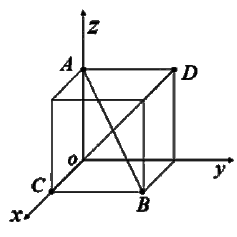
\includegraphics{pic/坐标系1.png}
    \caption{沿品胞基矢的方向建立坐标系。}
    \label{fig:1.2}
\end{figure}

所以,其夹角的余弦为:

\begin{align*}
    \cos\theta &= \frac{\overline{AB} \cdot \overline{CD}}{|\overline{AB}| \cdot |\overline{CD}|} \\
    \therefore \theta &= \arccos\left(-\frac{1}{3}\right) = \ang{109;28}
\end{align*}

\noindent \textbf{5.\quad} 试求面心立方结构 $(110)$ 和 $(111)$ 晶面族的原子数面密度,设晶格常数为 $a$。

\noindent \textbf{解:}

\begin{figure}[htbp]
    \centering
    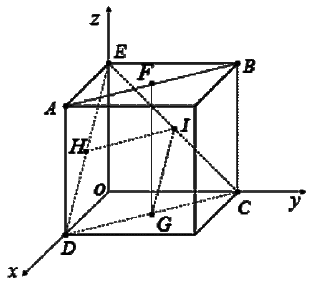
\includegraphics{pic/坐标系2.png}
    \caption{}
    \label{fig:1.3}
\end{figure}

如图所示,面 $ABCD$ 即 $(110)$ 面,面 $COE$ 即为 $(111)$ 面。设该面心立方的晶格常数为 $a$, 则在 $(110)$ 面内选取只包含一个原子的面 $AFGD$,其面积为 $a \cdot \frac{\sqrt{2}}{2} a=\frac{\sqrt{2}}{2} a^2$,所以其原子数面密度为

\begin{equation*}
    \frac{1}{\frac{\sqrt{2}}{2} a^2} = \frac{\sqrt{2}}{a^2}
\end{equation*}

在 $(111)$ 面内选取只包含一个原子的面 $DHIG$,其面积为:$\left(\frac{\sqrt{2}}{2}a\right)^2 \sin \frac{\pi}{3}=\frac{\sqrt{3}}{4} a^2$ 所以其原子数面密度为:

\begin{equation*}
    \frac{1}{\frac{\sqrt{3}}{4} a^2} = \frac{4\sqrt{3}}{3} a^2
\end{equation*}

\noindent \textbf{6.\quad} 若在面心立方结构的立方体心位置上也有一原子,试确定此结构的原胞,每个原胞内包含几个原子,设立方边长为 $a$。

\noindent \textbf{解:}

这种体心立方结构中有五种不同的原子。顶角、体心上的原子是两种不同的原子,另外,面心上的原子前后、上下、左右的原子两两一组,是互不相同的原子。故此种结构共有五种不同的原子,整个面心立方就是一个原胞。每个原胞中的原子数为:

\begin{equation*}
    8 \times \frac{1}{8} + 1 + 3 \times 2\times \frac{1}{2} = 5 (\text{个})
\end{equation*}

\noindent \textbf{7.\quad} 底心立方 (立方顶角与上、下底心处有原子)、侧心立方 (立方顶角与四个侧面的中心处有原子) 与边心立方 (立方顶角与十二条棱的中点有原子) 各属何种布拉维格子?每个原胞包含几个原子?

\noindent \textbf{解:}

这三种结构都属于简立方结构,原胞包含的原子数分别为:

\begin{enumerate}
    \item 底心立方:$\frac{1}{8} \times 8 = 1$
    \item 侧心立方:$\frac{1}{8} \times 8 + \frac{1}{2} \times 4 = 3$
    \item 边心立方:$\frac{1}{8} \times 8 + \frac{1}{4} \times 12 = 4$
\end{enumerate}

\noindent \textbf{8.\quad} 试证六角密集结构 $\frac{c}{a}=\sqrt{\frac{8}{3}}\approx 1.63$

\begin{figure}[htbp]
    \centering
    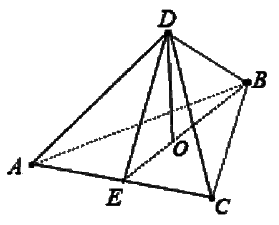
\includegraphics{pic/正四面体.png}
    \caption{正四面体}
    \label{fig:1.4}
\end{figure}

如图所示,$ABC$ 分别表示六角密集结构中中间层的三个原子,$D$ 表示底面中心的原子。$DABC$ 构成一个正四面体,为长为 $a$

$DO \perp \text{面} ABC$,则 $|DO|=\frac{c}{2}$

\begin{equation*}
    \because DE = \frac{\sqrt{3}}{2} a, \quad OE = \frac{1}{3} \cdot \frac{\sqrt{3}}{2} a = \frac{\sqrt{3}}{6} a
\end{equation*}

且 $DO \perp OE$,则由勾股定理可得

\begin{equation*}
    OD = \sqrt{\left(\frac{\sqrt{3}}{2}a\right)^2-\left(\frac{\sqrt{6}}{3}a\right)^2} = \frac{\sqrt{6}}{3} a
\end{equation*}

\begin{equation*}
    \therefore c = 2 OD = \frac{2\sqrt{6}}{3} a, \quad \frac{c}{a} = \frac{2\sqrt{6}}{3} = \sqrt{\frac{8}{3}} \approx 1.63
\end{equation*}
